\documentclass{ximera}

\usepackage{todonotes}

\newcommand{\RR}{\mathbb R}
\renewcommand{\d}{\,d}
\newcommand{\dd}[2][]{\frac{d #1}{d #2}}
\renewcommand{\l}{\ell}
\newcommand{\ddx}{\frac{d}{dx}}
\newcommand{\dfn}{\textbf}
\newcommand{\eval}[1]{\bigg[ #1 \bigg]}
\renewcommand{\epsilon}{\varepsilon}
\newcommand{\p}[1]{\left(#1\right)}
\newcommand{\br}[1]{\left[#1\right]}
\newcommand{\set}[1]{\left\{#1\right\}}


\let\prelim\lim
\renewcommand{\lim}{\displaystyle\prelim}

\colorlet{textColor}{black} 
\colorlet{background}{white}
\colorlet{penColor}{blue!50!black} % Color of a curve in a plot
\colorlet{penColor2}{red!50!black}% Color of a curve in a plot
\colorlet{penColor3}{red!50!blue} % Color of a curve in a plot
\colorlet{penColor4}{green!50!black} % Color of a curve in a plot
\colorlet{penColor5}{orange!80!black} % Color of a curve in a plot
\colorlet{fill1}{blue!50!black!20} % Color of fill in a plot
\colorlet{fill2}{blue!10} % Color of fill in a plot
\colorlet{fillp}{fill1} % Color of positive area
\colorlet{filln}{red!50!black!20} % Color of negative area
\colorlet{gridColor}{gray!50} % Color of grid in a plot


\newcommand{\fullwidth}{}
\newcommand{\normalwidth}{}



%% makes a snazzy t-chart for evaluating functions
\newenvironment{tchart}{\rowcolors{2}{}{background!90!textColor}\array}{\endarray}


\author{Gregory Hartman \and Matthew Carr}
\license{Creative Commons 3.0 By-NC}
\acknowledgement{https://github.com/APEXCalculus}

\begin{document}
\begin{exercise}

\outcome{Calculate limits using the limit laws.}

\tag{limit} 
\tag{quadratic} 
\tag{continuous}

  Find 
  \[
  \lim_{x\to 0} x^3-3x^2+x-5
  \begin{prompt}
  = \answer{-5}
  \end{prompt}
  \]
    \begin{hint}
      This function is continuous everywhere. Therefore, left-hand and right-hand limits exist at every point and are equal. Use this to your advantage by applying limit laws. Namely, the limit of a sum is the sum of the limits. Hence, 
    \[
    \lim_{x\to 0} \left( x^3-3x^2+x-5 \right)  
    = \lim_{x\to 0} \left( x^3 \right) +
    \lim_{x\to 0} \left( -3x^2 \right) +
    \lim_{x\to 0} \left( x \right) +
    \lim_{x\to 0} \left(-5\right).
    \]

    \end{hint}
     \begin{hint}
    Take a look at the graph of the function
    \begin{center}
     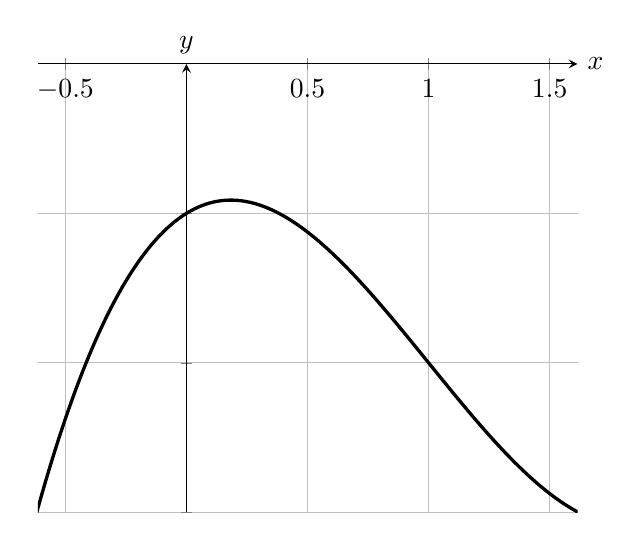
\begin{tikzpicture}
	\begin{axis}
	[ymin=-7,ymax=-4, axis lines=center,xlabel=$x$,ylabel=$y$,every axis y 
	label/.style={at=(current axis.above origin),anchor=south},every axis x label/.style={at=(current axis.right of origin),anchor=west},
	domain=-2:2,
	yticklabels={},
	ymajorgrids=true,
	grid = major
	]
	\addplot[very thick,smooth,samples=500]
	{\x^3-3*\x^2+\x-5};
	\end{axis}
       \end{tikzpicture}      
      \end{center}
    \end{hint}
    Additional limit laws imply that
    \[
    \lim_{x\to 0} \left( x^3-3x^2+x-5 \right)  
    = \left({\lim_{x\to 0} \left( x \right)}\right)^3 -
    3\cdot\lim_{x\to 0} \left( x^2 \right) +
    \lim_{x\to 0} \left( x \right) -
    \lim_{x\to 0} \left(5\right).
    \]
    \begin{hint}
     Evaluating $\lim_{x\to 0} \left( x^3-3x^2+x-5 \right)  
    = \left({\lim_{x\to 0} \left( x \right)}\right)^3 -
    3\cdot\lim_{x\to 0} \left( x^2 \right) +
    \lim_{x\to 0} \left( x \right) -
    \lim_{x\to 0} \left(5\right)$
    we see the answer is $5$, since, as we know, $\lim_{x\to0}\left({x}\right)=0$.
     \end{hint}
    
\end{exercise}
\end{document}